\documentclass[11pt, oneside]{article}   	% use "amsart" instead of "article" for AMSLaTeX format
\usepackage{geometry}                		% See geometry.pdf to learn the layout options. There are lots.
\geometry{letterpaper}                   		% ... or a4paper or a5paper or ... 
\usepackage[parfill]{parskip}    		% Activate to begin paragraphs with an empty line rather than an indent
\usepackage{graphicx}				% Use pdf, png, jpg, or eps§ with pdflatex; use eps in DVI mode
								% TeX will automatically convert eps --> pdf in pdflatex		
\usepackage{amssymb}
\usepackage{amsmath}
\usepackage[
backend=biber,
style=alphabetic,
]{biblatex}
\usepackage{graphicx}
\graphicspath{ {./images/} }
\usepackage{verbatim}
\usepackage{tikz} 

\usepackage{syntonly}
% \syntaxonly <-- use this for checking syntax only
% \mbox {text} - keep together
% \fbox {text} - keep together and draw around

%\pagestyle{plain|headings|empty} % header and footer p.27
%SetFonts
%\include{filename}, \includeonly{filename1, filename2} , \input[fiename}

%SetFonts% 

\title{Solving N-dle using Information Entropy}
\author{Dave Fetterman}
\date{6/1/22}							% Activate to display a given date or no date

\begin{document}
\maketitle
\section{Introduction}

\begin{itemize}
\item Introduce Entropy and Alex's paper.  
\item Reducing 2309 possibilities to one within five moves requires eliminating large portions of the dictionary with each move. 
\item  TODO: Summarize algorithm.
\end{itemize}

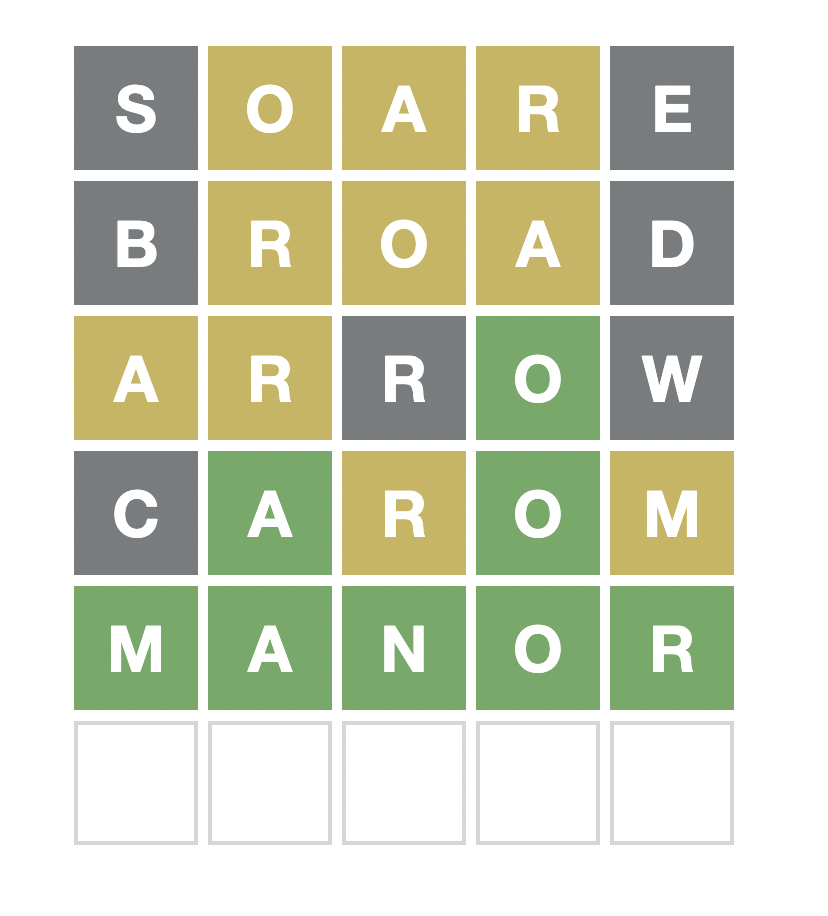
\includegraphics[scale=.5]{wordle}

  For the likely reader, Wordle needs no introduction. As Mastermind with a restricted solution set (an English dictionary restricted to a reduced set of five-letter words), the sharing and scarcity aspects of the game led to its viral spread, various knockoffs, and ultimate purchase by the New York Times.
  
  
  - With six guesses to determine the mystery word, each turn yields information in the form of Green, Yellow, and Black squares.  At any given slot of five:
     - A green square indicates the guess has the correct letter in that slot.
     - A yellow square indicates the guessed letter does not match the solution in this slot, but exists elsewhere in the solution.
     - A black square indicates the guessed letter does not match the solution in this slot, and there are no more instances of this letter in the solution.   
     - If the solution has five unique letters, the above rules are straightforward to interpret.
     - If the solution has repeated letters, note that, for any letter:
       - All yellow squares appear before all black squares.
       - The number of green and yellow squares don't exceed the number of instances of the letter in the soluton.
      - In the current dictionary, triple lettes include bobby, daddy, eerie, emcee, geese, melee, tepee, fluff, mamma, mammy, mummy, nanny, ninny, pappy, puppy, error, rarer, sassy, sissy, and tatty (20 words).
  - Starting with a well-known dictionary of 2309 words (link), the player has six guesses to enter the correct word (that is, receive all greens as a response).  
  - Again, this is just like Mastermind, except that TWO dictionaries play a large role:
     - All answers come from the answers dictionary (TODO github link), with 2309 entires.
     - All allowed guesses come from the guesses dictionary (TODO github link), with 129
     
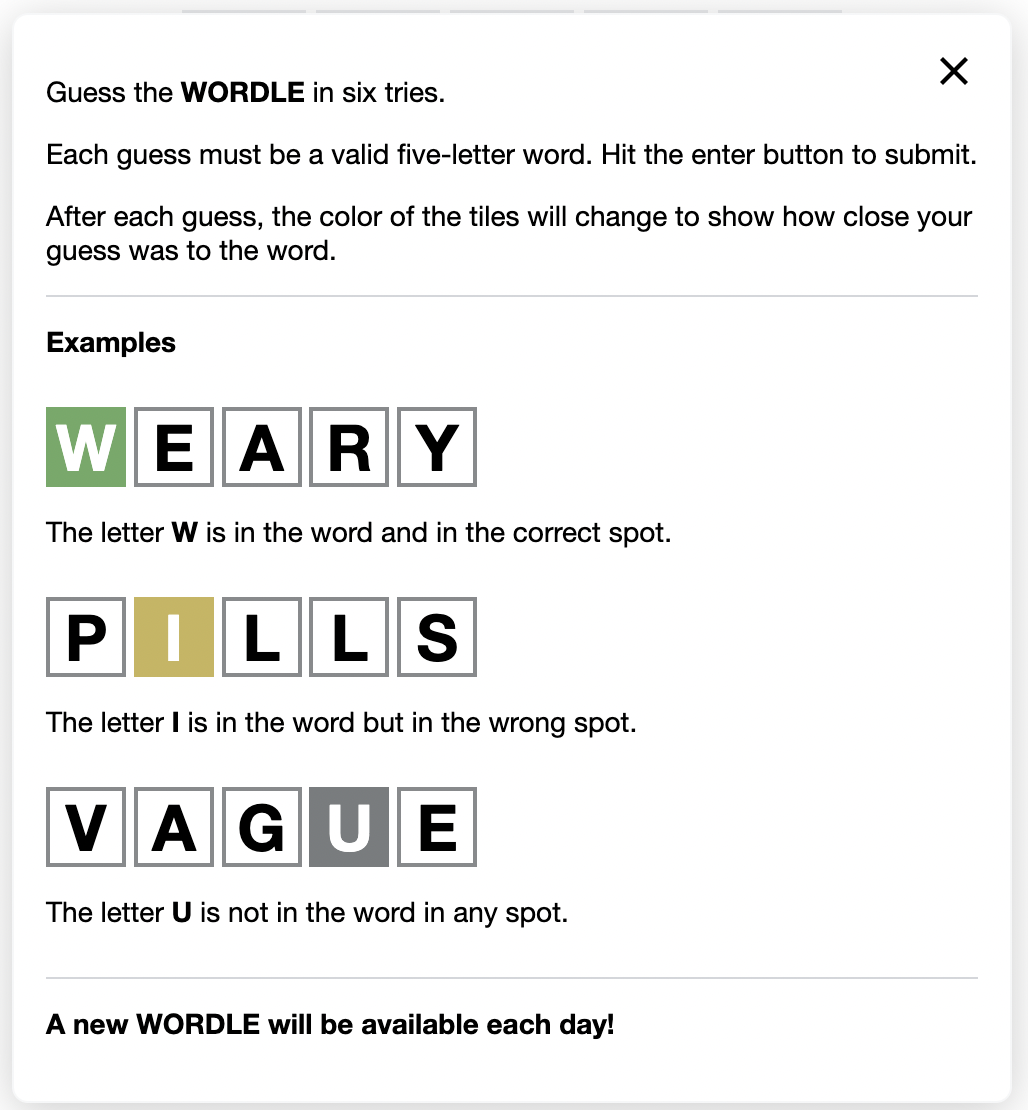
\includegraphics[scale=.5]{rules}

\section{Considering Entropy}
\begin{itemize}
\item - Entropy negatives: heuristic, greedy, may miss EV.
\item Entropy positive: scales across independent events.
\item Define independent events in n-dle
\end{itemize}

\section{N-dle using entropy}
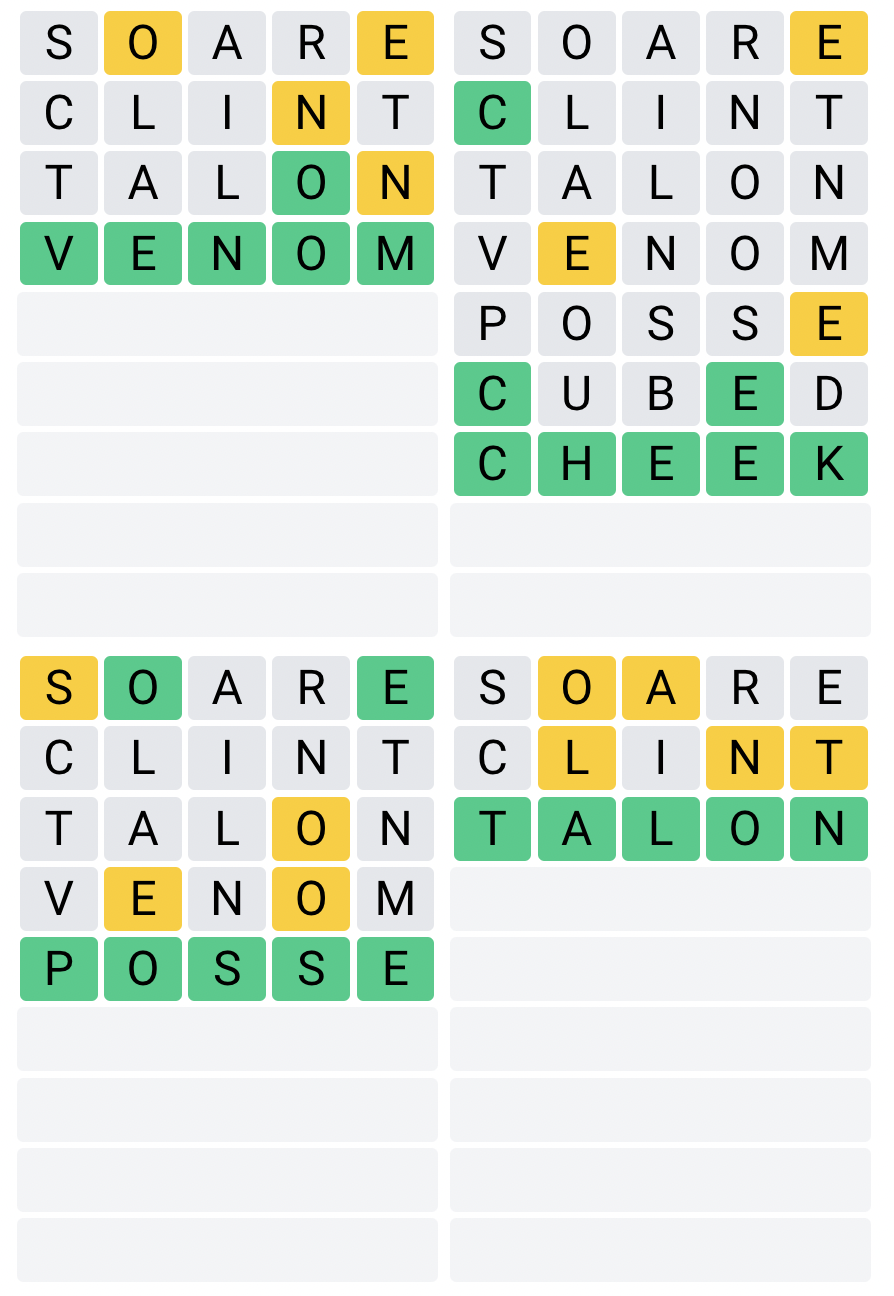
\includegraphics[scale=.5]{quordle}

TEXT

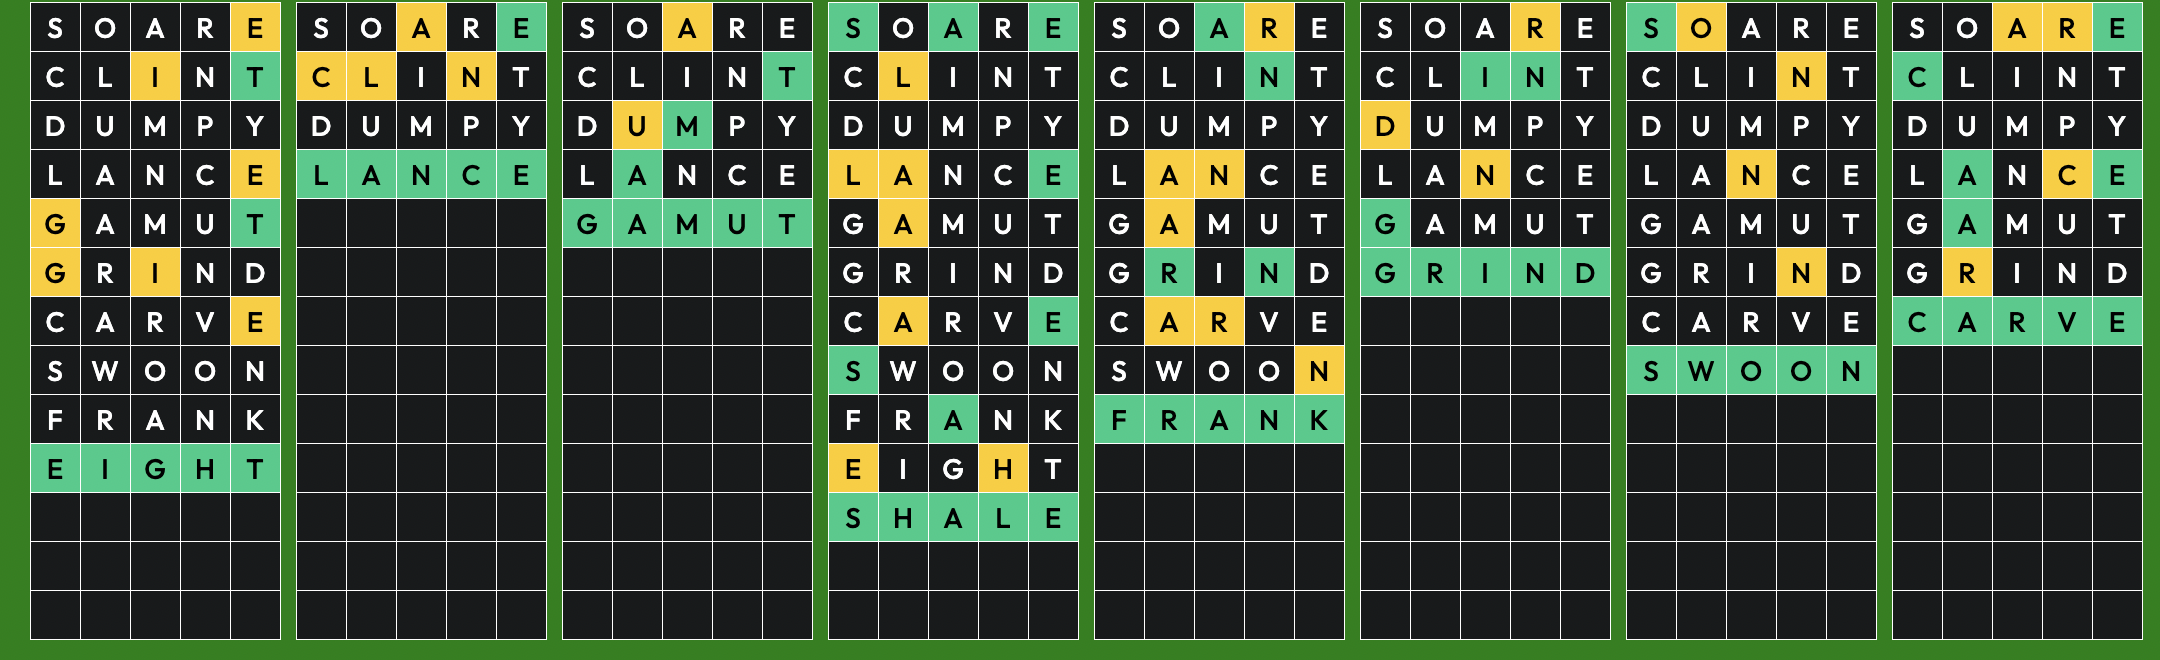
\includegraphics[width=\textwidth]{octordle}


\begin{itemize}
\item - Entropy negatives: heuristic, greedy, may miss EV.
\item Entropy positive: scales across independent events.
\item Define independent events in n-dle
\item Greedy on solve - moot in wordle, but always take the solution; you'll have to spend anyway and you're receiving less info later.
 \item Sum across all
\end{itemize}

\section{Experimental Results}
\begin{itemize}
 \item Necesasrily trends to N+0
\item Starts at about N+3
\item How effective is starting with the same two words?
\end{itemize}

\section{Caveats}
\begin{itemize}
\item 
\item Ties are arbitrary but likely not uniformly random
\item  Doesn't play "endgames" well.  
\item What's the link between reducing entropy as 
\end{itemize}

\section{Remaining Questions}
\begin{itemize}
\item TODO
\end{itemize}

\section{First section}

Items that are cited: \textit{The \LaTeX\ Companion} book \cite{latexcompanion} together with Einstein's journal paper \cite{einstein} and Dirac's book \cite{dirac}---which are physics-related items. Next, citing two of Knuth's books: \textit{Fundamental Algorithms} \cite{knuth-fa} and \textit{The Art of Computer Programming} \cite{knuth-acp}.

\cite{lamport94} is a set of macros built atop \TeX{} \cite{1}.

\begin{thebibliography}{9}
\bibitem{1}
Claude Shannon (1948) \emph{A Mathematical Theory of Communication}. Bell System Technical Journal 27, 379-423.
\bibitem{2}
Alex Healy \emph{On Optimal Strategies for Wordle}, \url{http://www.alexhealy.net/papers/wordle.pdf}.
\bibitem{3}
Thomas M. Cover; Joy A. Thomas (1991). \emph{Elements of Information Theory}, retrieved from \url{https://en.wikipedia.org/wiki/Entropy_(information_theory}
\end{thebibliography}

\end{document}
